% !TeX root = main.tex

\chapter{随机变量及其分布}
\thispagestyle{plain}

\section{随机变量及其分布函数}

\subsection{随机变量}

\begin{definition}
    \indent 设随机试验 $E$ 的样本空间为 $\varOmega=\{\omega\}$. 如果对于每一个 $\omega\in\varOmega$,都有一个实数 $X(\omega)$ 与之对应,则称 $X=X(\omega)$ 为\textbf{随机变量}(random variable).
\end{definition}

随机变量常用大写字母 $X,Y,Z$ 等表示.

\subsection{分布函数}

\begin{definition}
    \indent 设 $X$ 是一个随机变量,对于任意实数 $x$,令
    $$
    F(x)=P(X \leqslant x), \ x \in \mathbf{R}
    $$
    称 $F(x)$ 为随机变量 $X$ 的\textbf{分布函数}(cumulative distribution function).称随机变量 $X$ 服从 $F(x)$,记为 $X \sim F(x)$.
\end{definition}

随机变量 $X$ 的分布函数 $F(x)$ 是定义在 $(-\infty, +\infty)$ 上的函数,是随机事件 $\{X \leqslant x\}$ 发生的概率.分布函数值 $F(a)$ 表示 $X$ 落在区间 $(-\infty,a]$ 上的概率.

\begin{property}[][单调性]
    \indent $F(x)$ 是一个单调不减函数,即对任意的 $x_1 < x_2$,有 $F(x_1) \leqslant F(x_2)$.
\end{property}

\begin{proof}
    对于任意实数 $x_1, x_2\, (x_1 < x_2)$,有
    $$
    F(x_2) - F(x_1) = P(x_1 < X \leqslant x_2) \geqslant 0
    $$
    因此 $F(x)$ 是单调不减函数.
\end{proof}

\begin{property}[][有界性]
    \indent 对于任意实数 $x$,有 $0 \leqslant F(x) \leqslant 1$,且
    \begin{gather*}
        F(-\infty)= \lim_{x \to -\infty} F(x) = 0 \\
        F(+\infty)= \lim_{x \to +\infty} F(x) = 1
    \end{gather*}
\end{property}

\begin{proof}
    因为 $F(x) = P(X \leqslant x)$,根据概率的性质可得 $0 \leqslant F(x) \leqslant 1$.

    $F(x)$ 在 $(-\infty, +\infty)$ 内单调不减且有界,由单调有界原理可知,$\displaystyle\lim_{x \to -\infty} F(x)$ 和 $\displaystyle\lim_{x \to +\infty} F(x)$ 存在.

    记 $A_n = \{ X \leqslant n \}$,则有 $A_n \subseteq A_{n+1}$,$\displaystyle\bigcup_{i=1}^{\infty} A_i = \varOmega$.由海涅定理可得
    $$
    \lim_{x \to +\infty} F(x) = \lim_{n \to \infty} F(n) = \lim_{n \to \infty} P(A_n) = P(\lim_{n \to \infty} A_n) = P \left( \bigcup_{i=1}^{\infty} A_i \right) = 1
    $$

    记 $B_n = \{ X \leqslant -n \}$,则有 $B_n \supseteq B_{n+1}$,$\displaystyle\bigcap_{i=1}^{\infty} B_i = \text{\O}$.由海涅定理可得
    $$
    \lim_{x \to -\infty} F(x) = \lim_{n \to \infty} F(-n) = \lim_{n \to \infty} P(B_n) = P(\lim_{n \to \infty} B_n) = P \left( \bigcap_{i=1}^{\infty} B_i \right) = 0
    $$

    \vspace{-2em}
\end{proof}

\begin{property}[][右连续性]
    \indent $F(x)$ 处处右连续,即对任意实数 $x_0$,有 $F(x_0^+) = F(x_0)$.
\end{property}

\begin{proof}
    因为 $F(x)$ 是单调不减有界函数,所以对任意实数 $x_0$,右极限 $F(x_0^+)$ 一定存在.记 $A_n = \{ X \leqslant x_0 + \dfrac{1}{n} \}$,则有 $A_n \supseteq A_{n+1}$,$\displaystyle\bigcap_{i=1}^{\infty} A_i = \{ X \leqslant x_0 \}$,由海涅定理得
    $$
    \begin{aligned}
        \lim_{x \to x_0^+} F(x) &= \lim_{n \to \infty} F(x_0 + \dfrac{1}{n}) \\
        &= \lim_{n \to \infty} P(A_n) \\
        &= P(\lim_{n \to \infty} A_n) \\
        &= P \left( \bigcap_{i=1}^{\infty} A_i \right) \\
        &= P(X \leqslant x_0) \\
        &= F(x_0)
    \end{aligned}
    $$

    \vspace{-1em}
\end{proof}

单调性、有界性、右连续性是分布函数的基本性质.分布函数一定具有这些基本性质,反过来,满足这些基本性质的函数一定是某个随机变量的分布函数.因此,这三条基本性质是判定某个函数能否成为分布函数的充分必要条件.

\begin{property}
    \indent 对于任意实数 $x_1,x_2\, (x_1<x_2)$,有 $P(x_1 < X \leqslant x_2)=F(x_2)-F(x_1)$.
\end{property}

\begin{proof}
    对于任意实数 $x_1,x_2\, (x_1<x_2)$,由于
    $$
    \{x_1 < X \leqslant x_2\} = \{X \leqslant x_2\} - \{X \leqslant x_1\}
    $$
    所以有
    $$
    \begin{aligned}
        P(x_1 < X \leqslant x_2) &= P(X \leqslant x_2) - P(X \leqslant x_1) \\
        &= F(x_2)-F(x_1)
    \end{aligned}
    $$

    \vspace{-1.5em}
\end{proof}

\section{离散型随机变量及其概率分布}

\begin{definition}
    \indent 如果一个随机变量 $X$ 所有可能取到的不相同的值是有限个或可列无限多个,并且以确定的概率取这些不同的值,则称 $X$ 为\textbf{离散型随机变量}(discrete random variable).
\end{definition}

\begin{definition}
    \indent 设离散型随机变量 $X$ 所有可能取的值为 $x_k\, (k=1,2,\cdots)$,$X$ 取各个可能值的概率,即事件 $\{X=x_k\}$ 的概率为
    \begin{equation} \label{equation:distribution}
        P(X=x_k) = p_k, \ k=1,2,\cdots
    \end{equation}
    并且 $p_k$ 满足以下两个条件:
    \begin{enumerate}
        \item 非负性:$p_k \geqslant 0$;\vspace{0.5em}
        \item 归一性:$\displaystyle\sum_{k=1}^\infty p_k = 1$,
    \end{enumerate} \vspace{0.5em}
    则称式 \eqref{equation:distribution} 为离散型随机变量 $X$ 的\textbf{概率分布}(probability distribution)或\textbf{分布律}.
\end{definition}

概率分布也可以用如下的表格来表示:
\begin{table*}[htbp]
    \centering

    \begin{tabular}{c | c c c c c}
        \hline
        $X$ & $x_1$ & $x_2$ & $\cdots$ & $x_k$ & $\cdots$ \\
        \hline
        $P$ & $p_1$ & $p_2$ & $\cdots$ & $p_k$ & $\cdots$ \\
        \hline
    \end{tabular}
\end{table*}

概率分布反映了离散型随机变量的统计规律性.

对于任意实数 $x$,随机事件 $\{X \leqslant x\}$ 可以表示成 $\displaystyle\bigcup_{x_k \leqslant x} \{X=x_k\}$. 由于 $x_k\, (k=1,2,\cdots)$ 互不相同,根据概率的可加性,可得离散型随机变量 $X$ 的分布函数为
$$
F(x) = P(X \leqslant x) = \sum_{x_k \leqslant x} P(X=x_k) = \sum_{x_k \leqslant x} p_k
$$
它的图像是有限级(或可列无限级)的阶梯形曲线.

如果随机变量 $X$ 只能取一个常数 $c$,即 $P(X=c) = 1$,这样的分布称为\textbf{单点分布}或\textbf{退化分布},它的分布函数是
$$
F(x) = \begin{cases}
    0, & x < c \\
    1, & x \geqslant c
\end{cases}
$$

\section{连续型随机变量及其概率密度}

\begin{definition}[][][def:f(x)]
    \indent 对于随机变量 $X$ 的分布函数 $F(x)$,如果存在非负函数 $f(x)$,使得对任意的 $x$,都有 $F(x)=\displaystyle\int_{-\infty}^x f(t)\,\text{d}t$,则称随机变量 $X$ 是\textbf{连续型随机变量}(continuous random variable),其中函数 $f(x)$ 叫做 $X$ 的\textbf{概率密度函数}(probability density function),简称为\textbf{概率密度}(probability density),记作 $X \sim f(x)$.
\end{definition}

由定义 \ref{def:f(x)} 可知,连续型随机变量的分布函数处处连续.

\vspace{0.2em}

\begin{property}[][非负性][prop:f(x)>=0]
    \indent $f(x) \geqslant 0$
\end{property}

\begin{property}[][规范性][prop:f(x):integral=1]
    \indent $\displaystyle\int_{-\infty}^{+\infty} f(x)\,\text{d}x = 1$
\end{property}

非负性和规范性是概率密度函数的基本性质.概率密度函数一定具有这两个性质,满足这两个性质的函数也一定是某随机变量的概率密度.因此,非负性和规范性是判断某个函数能否作为概率密度函数的充分必要条件.

\begin{property}
    \indent 对于任意实数 $a,b\,(a<b)$,有
    $$
    P(a < X \leqslant b) = F(b)-F(a) = \int_a^b f(x)\,\text{d}x
    $$
\end{property}

由以上性质可知,概率密度曲线总是位于 $x$ 轴上方,并且介于它和 $x$ 轴之间的面积等于 $1$;随机变量落在区间 $(a,b]$ 的概率 $P(a < X \leqslant b)$ 等于区间 $(a,b]$ 上曲线 $y=f(x)$ 之下的曲边梯形的面积.

\begin{property}[][][prop:F'(x)=f(x)]
    \indent 如果 $f(x)$ 在点 $x$ 处连续,则有 $F'(x)=f(x)$.
\end{property}

由性质 \ref{prop:F'(x)=f(x)} 可知,在 $f(x)$ 的连续点有
$$
\begin{aligned}
    f(x) &= \lim_{\Delta x \to 0^+} \dfrac{F(x + \Delta x)-F(x)}{\Delta x}\\
    &= \lim_{\Delta x \to 0^+} \dfrac{P(x < X \leqslant x + \Delta x)}{\Delta x}
\end{aligned}
$$
可见概率密度反映了随机变量在点 $x$ 处概率分布的密集程度.$f(x)$ 的大小能反映出随机变量 $X$ 在点 $x$ 附近取值的可能性大小,即概率的大小.因此,用概率密度描述连续型随机变量的分布比用分布函数更直观.当不考虑高阶无穷小时,有
$$
P(x < X \leqslant x + \Delta x) \approx f(x) \Delta x
$$

\begin{conclusion}
    \indent 连续型随机变量取任意指定实数的概率均为零.
\end{conclusion}

\begin{proof}
    对于 $X$ 的任意一个可取的值 $x$,设 $\Delta x > 0$,由于事件 $\{X=x\} \subseteq \{x - \Delta x < X \leqslant x\}$,因此有
    $$
    0 \leqslant P(X=x) \leqslant P(x - \Delta x < X \leqslant x) = F(x)-F(x-\Delta x)
    $$
    令 $\Delta x \to 0$,可得
    $$
    P(X=x)=0
    $$
    因此,连续型随机变量取任意指定实数的概率均为零.
\end{proof}

据此,在计算连续型随机变量在某一区间取值的概率时,可以不区分该区间是开区间或闭区间或半开半闭区间,即有
$$
P(x_1 < X < x_2) = P(x_1 \leqslant X \leqslant x_2) = P(x_1 < X \leqslant x_2) = P(x_1 \leqslant X < x_2) = \int_{x_1}^{x_2} f(x)\,\text{d}x
$$

由上述结论可知,不可能事件的概率为 $0$,但概率为 $0$ 的事件未必是不可能事件.类似地,必然事件的概率为 $1$,但概率为 $1$ 的事件未必是必然事件.

\begin{note}
    \indent 由于在若干点上改变概率密度 $f(x)$ 的值并不影响其积分的值,从而不影响其分布函数 $F(x)$ 的值,这意味着一个连续型概率分布的概率密度不唯一.例如:
    $$
    f_1(x) = \begin{cases}
        \dfrac{1}{a}, & 0 \leqslant x \leqslant a \\[0.3em]
        0, & \text{其他} \\
    \end{cases}
    \qquad
    f_2(x) = \begin{cases}
        \dfrac{1}{a}, & 0 < x < a \\[0.3em]
        0, & \text{其他}
    \end{cases} \\
    $$
    这两个概率密度只在 $x=0$ 和 $x=a$ 处的取值不同,因此
    $$
    P(f_1(x) \not= f_2(x)) = P(X=0) + P(X=a) = 0
    $$
    可见这两个函数在概率意义上没有差别,称 $f_1(x)$ 与 $f_2(x)$ “几乎处处相等”,其意义是:在概率论中可除去概率为 $0$ 的事件后讨论两个函数相等和其他随机问题.
\end{note}

\begin{note}
    \indent 除了离散型概率分布和连续型概率分布之外,还有既非离散又非连续的分布.例如:
    $$
    F(x) = \begin{cases}
        0, & x<0 \\
        \dfrac{x+1}{2}, & 0 \leqslant x < 1 \\
        1, & x \geqslant 1
    \end{cases}
    $$
    $F(x)$ 是一个分布函数,它既不是阶梯函数,也不是连续函数,所以它既不是离散型概率分布,又不是连续型概率分布.这是一种新的分布,这类分布函数通常可以分解为两个分布函数的凸组合,如上述 $F(x)$ 可分解为
    $$
    F(x) = \dfrac{1}{2} F_1(x) + \dfrac{1}{2} F_2(x)
    $$
    其中
    $$
    F_1(x) = \begin{cases}
        0, & x<0 \\
        1, & x \geqslant 0
    \end{cases}
    \qquad
    F_2(x) = \begin{cases}
        0, & x<0 \\
        x, & 0 \leqslant x < 1 \\
        1, & x \geqslant 1
    \end{cases}
    $$
    而 $F_1(x)$ 是离散型概率分布(单点分布)的分布函数,$F_2(x)$ 是连续型概率分布(均匀分布)的分布函数.
\end{note}

\section{常用的概率分布}

\subsection{0-1分布}

\begin{definition}
    \indent 如果离散型随机变量 $X$ 只取 $0$ 与 $1$ 两个值,其概率分布为
    $$
    P(X=0)=1-p, \; P(X=1)=p, \; 0<p<1
    $$
    或写成
    $$
    P(X=k)=p^k (1-p)^{1-k}, \; k=0,1, \; 0<p<1
    $$
    则称随机变量 $X$ 服从参数为 $p$ 的\textbf{0-1分布}或\textbf{两点分布}(two-point distribution).
\end{definition}

服从两点分布的随机变量 $X$ 的概率分布也可以写成
\begin{table*}[htbp]
    \centering

    \begin{tabular}{c | c c}
        \hline
        $X$ & 0 & 1 \\
        \hline
        $P$ & $1-p$ & $p$ \\
        \hline
    \end{tabular}
\end{table*}

\subsection{二项分布}

在 $n$ 重伯努利试验中,如果以 $X$ 表示事件 $A$ 出现的次数,则 $X$ 是一个离散型随机变量,它的所有可能取值是 $0,1,2,\cdots,n$.设 $P(A)=p\,(0<p<1)$,则由二项概率公式(式 \eqref{equation:binomial})可得
$$
P(X=k)=C_n^k p^k (1-p)^{n-k}, \; k=0,1,\cdots,n
$$

\begin{definition}[][][def:binomial distribution]
    \indent 如果随机变量 $X$ 的概率分布为
    $$
    P(X=k)=C_n^k p^k (1-p)^{n-k}, \; k=0,1,\cdots,n
    $$
    则称随机变量 $X$ 服从参数为 $n,p$ 的\textbf{二项分布}(binomial distribution),记作 $X \sim B(n,p)$.
\end{definition}

由定义 \ref{def:binomial distribution} 可得
\begin{gather*}
    P(X=k) \geqslant 0\\
    \sum_{k=0}^n P(X=k) = \sum_{k=0}^n C_n^k p^k (1-p)^{n-k} = [p+(1-p)]^n=1
\end{gather*}

特别地,当 $n=1$ 时,二项分布 $B(1,p)$ 的概率分布为
$$
P(X=k) = p^k (1-p)^{1-k}, \; k=0,1
$$
这就是0-1分布. 因此,0-1分布是二项分布的特例.

在 $n$ 重伯努利试验中,设第 $i$ 次试验中 $A$ 出现的次数为 $X_i$,则 $X_i$ 服从0-1分布.由于 $n$ 次试验相互独立,所以产生的 $n$ 个随机变量 $X_1, X_2, \cdots, X_n$ 也相互独立,将它们加起来,得到新的随机变量
$$
X = X_1 + X_2 + \cdots + X_n
$$
$X$ 就是 $n$ 重伯努利试验中 $A$ 出现的总次数,它服从二项分布 $B(n,p)$.因此,服从二项分布的随机变量总可以分解成 $n$ 个相互独立且同为0-1分布的随机变量之和.

\subsection{泊松分布}

\begin{definition}
    \indent 如果离散型随机变量 $X$ 的所有可能取值为 $0,1,2,\cdots$,并且
    $$
    P(X=k) = \dfrac{\lambda^k e^{-\lambda}}{k!}, \; k=0,1,2\cdots
    $$
    其中 $\lambda > 0$ 是常数,则称随机变量 $X$ 服从参数为 $\lambda$ 的\textbf{泊松分布}(poisson distribution),记作 $X \sim P(\lambda)$ 或 $X \sim \pi(\lambda)$.
\end{definition}

由定义可知
\begin{gather*}
    \dfrac{\lambda^k e^{-\lambda}}{k!} > 0 \\
    \sum_{k=0}^\infty \dfrac{\lambda^k e^{-\lambda}}{k!} = e^{-\lambda} \sum_{k=0}^\infty \dfrac{\lambda^k}{k!} = e^{-\lambda} e^{\lambda} = 1
\end{gather*}

\begin{figure}[htbp]
    \centering

    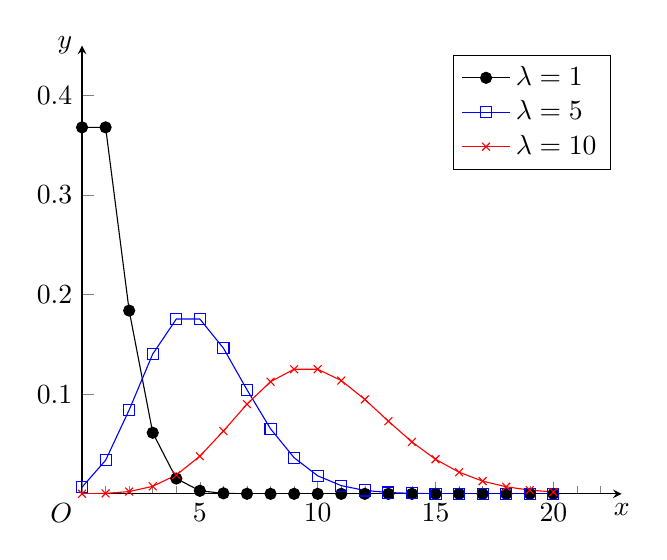
\begin{tikzpicture}
        \begin{axis}[xlabel=$x$, ylabel=$y$,
            axis lines=center,
            tick align=inside,
            xtick distance=5, ytick distance=0.1,
            minor x tick num=4,
            xmin=0, xmax=22.9,
            ymin=0, ymax=0.45,
            every axis x label/.style={
                at={(xticklabel* cs:1)},
                anchor=north
            },
            every axis y label/.style={
                at={(yticklabel* cs:1)},
                anchor=east
            },
            legend style={
                cells={anchor=west}
            },
            extra x ticks={0},
            extra x tick label={$O$},
            extra x tick style={
                tick label style={anchor=north east}
            }
        ]
            \addplot[domain=0:20, samples=21, mark=*]{exp(-1)/(x!)};
            \addplot[domain=0:20, samples=21, mark=square, color=blue]{5^x * exp(-5) / (x!)};
            \addplot[domain=0:20, samples=21, mark=x, color=red]{10^x * exp(-10) / (x!)};

            \legend{$\lambda=1$, $\lambda=5$, $\lambda=10$}
        \end{axis}
    \end{tikzpicture}

    \caption{泊松分布}
\end{figure}

\begin{theorem}[][泊松定理]
    \indent 设 $\{ p_n \}$ 为一个实数序列,且对于任意正整数 $n$,有 $p_n \in [0,1]$.若 $n \to \infty$ 时有 $n p_n \to \lambda$($\lambda > 0$),则对任一固定的非负整数 $k$,有
    $$
    \lim_{n\to\infty} C_n^k p_n^k (1-p_n)^{n-k} = \dfrac{\lambda^k e^{-\lambda}}{k!}
    $$
\end{theorem}

\begin{proof}
    记 $n p_n=\lambda_n$,即 $p_n=\dfrac{\lambda_n}{n}$,从而对于任意固定的非负整数 $k$,有
    $$
    \begin{aligned}
        & C_n^k p_n^k (1-p_n)^{n-k} \\
        =\ & \dfrac{n(n-1) \cdots (n-k+1)}{k!} \left( \dfrac{\lambda_n}{n} \right)^k \left( 1-\dfrac{\lambda_n}{n} \right)^{n-k} \\
        =\ & \dfrac{\lambda_n^k}{k!} \left[ \left( 1-\dfrac{1}{n} \right) \left( 1-\dfrac{2}{n} \right) \cdots \left( 1-\dfrac{k-1}{n} \right) \right] \left( 1-\dfrac{\lambda_n}{n} \right)^n \left( 1-\dfrac{\lambda_n}{n} \right)^{-k}
    \end{aligned}
    $$
    对于固定的 $k$,有
    $$
    \begin{aligned}
        & \lim_{n \to \infty} \lambda_n = \lambda \\
        & \lim_{n \to \infty} \left( 1-\dfrac{1}{n} \right) \left( 1-\dfrac{2}{n} \right) \cdots \left( 1-\dfrac{k-1}{n} \right) = 1 \\
        & \lim_{n \to \infty} \left( 1-\dfrac{\lambda_n}{n} \right)^n = e^{-\lambda} \\
        & \lim_{n \to \infty} \left( 1-\dfrac{\lambda_n}{n} \right)^{-k} = 1 \\
    \end{aligned}
    $$
    所以
    $$
    \lim_{n\to\infty} C_n^k p_n^k (1-p_n)^{n-k} = \dfrac{\lambda^k e^{-\lambda}}{k!}
    $$
\end{proof}

对于二项分布 $B(n,p)$,$np$ 为定值,当 $n$ 很大而 $p$ 很小时,$np = \lambda$ 大小适中,可以将二项分布近似为泊松分布.

\subsection{几何分布}

设试验 $E$ 只有两个对立的结果 $A$ 和 $\overline{A}$,并且 $P(A)=p, \, P(\overline{A})=1-p$,其中 $0<p<1$. 将试验 $E$ 独立地重复进行下去,直到事件 $A$ 发生为止. 如果用 $X$ 表示所需要的试验次数,则 $X$ 是一个离散型随机变量,它的所有可能取值为 $1,2,3,\cdots$,其概率分布为
$$
P(X=k) = (1-p)^{k-1} p, \; k=1,2,\cdots
$$
称随机变量 $X$ 服从参数为 $p$ 的\textbf{几何分布}(geometric distribution),记作 $X \sim Ge(p)$.

易知
\begin{gather*}
    (1-p)^{k-1} p > 0 \\
    \sum_{k=1}^\infty (1-p)^{k-1} p = p \sum_{i=0}^\infty (1-p)^i = p \cdot \dfrac{1}{1-(1-p)} = 1    
\end{gather*}

\begin{theorem}[][几何分布的无记忆性][theorem:几何分布的无记忆性]
    \indent 设 $X \sim Ge(p)$,则对任意正整数 $m$ 与 $n$,有
    \begin{equation}
        P(X > m+n \mid X>m) = P(X>n)
    \end{equation}
\end{theorem}

\begin{proof}
    因为
    $$
    P(X>n) = \sum_{k=n+1}^{\infty} (1-p)^{k-1} p = \dfrac{p (1-p)^n}{1-(1-p)} = (1-p)^n
    $$
    所以对任意正整数 $m$ 与 $n$,有
    $$
    P(X > m+n \mid X>m) = \dfrac{P(X > m+n)}{P(X>m)} = \dfrac{(1-p)^{m+n}}{(1-p)^m} = (1-p)^n = P(X>n)
    $$

    \vspace{-2em}
\end{proof}

\begin{note}
    \indent 若 $X \sim Ge(p)$,则事件 $\{ X>m \}$ 表示前 $m$ 次试验中 $A$ 没有出现.假如在接下去的 $n$ 次试验中 $A$ 仍未出现,这个事件记为 $\{ X > m+n \}$.定理 \ref{theorem:几何分布的无记忆性} 表明,在前 $m$ 次试验中 $A$ 没有出现的条件下,接下去的 $n$ 次试验中 $A$ 仍未出现的概率只与 $n$ 有关,而与之前的 $m$ 次试验无关,这就是无记忆性.
\end{note}

\subsection{超几何分布}

设有 $N$ 件物品,其中有 $M$($M \leqslant N$) 件为甲类,从中不放回地随机抽取 $n$($n \leqslant N$) 件,记抽出甲类物品的数量为 $X$,则随机变量 $X$ 服从\textbf{超几何分布}(hypergeometric distribution),记为 $X \sim H(n,N,M)$.

当 $n \leqslant N-M$ 时,$X$ 的取值范围为 $0,1,2,\cdots,\min\{ M,n \}$;当 $n > N-M$ 时,一定能够抽出甲类物品,$X$ 的取值范围为 $n+M-N, n+M-N+1, n+M-N+2, \cdots, \min\{ M,n \}$.综合两种情况,记 $m = \max\{ 0, n+M-N \}$,$r = \min\{ M,n \}$,则超几何分布的概率分布为
$$
P(X=k) = \dfrac{C_M^k C_{N-M}^{n-k}}{C_N^n},\ k=m, m+1, m+2, \cdots, r
$$

\begin{note}
    \indent 当 $N=M$ 时,有
    $$
    P(X=n) = \dfrac{C_M^n C_{N-M}^{n-n}}{C_N^n} = C_0^0 = 1
    $$
    $C_0^0$ 本身没有意义,但为了保证组合数定义的一致性,规定 $C_0^0 = 1$.
\end{note}

当 $n \ll N$ 时,每次抽取后,甲类物品所占比例 $p = \dfrac{M}{N}$ 改变很小,此时可以将不放回抽样近似看做放回抽样,超几何分布近似为二项分布:
$$
\dfrac{C_M^k C_{N-M}^{n-k}}{C_N^n} \approx C_n^k p^k (1-p)^{n-k}
$$

\subsection{帕斯卡分布}

设试验 $E$ 只有两个对立的结果 $A$ 和 $\overline{A}$,并且 $P(A)=p, \, P(\overline{A})=1-p$,其中 $0<p<1$. 将试验 $E$ 独立地重复进行下去,记事件 $A$ 第 $r$ 次出现时的试验次数为 $X$,则 $X$ 的可能取值为 $r, r+1, r+2, \cdots$,称随机变量 $X$ 服从\textbf{帕斯卡分布}(Pascal distribution).

帕斯卡分布是\textbf{负二项分布}(negative binomial distribution)的正整数形式,因此可以将帕斯卡分布记作 $X \sim Nb(r,p)$.

如果 $X=k$,意味着第 $k$ 次试验时事件 $A$ 第 $r$ 次出现,而前 $k-1$ 次试验中 $A$ 出现 $r-1$ 次,由二项分布知
$$
P(X=k) = C_{k-1}^{r-1} p^{r-1} (1-p)^{k-r} \cdot p
$$
因此帕斯卡分布的概率分布为
$$
P(X=k) = C_{k-1}^{r-1} p^r (1-p)^{k-r},\ k = r, r+1, r+2, \cdots
$$

当 $r=1$ 时,帕斯卡分布即为几何分布.

如果将第一个 $A$ 出现的试验次数记为 $X_1$,第二个 $A$ 出现的试验次数记为 $X_2$(从第一个 $A$ 出现之后算起),$\cdots$,第 $r$ 个 $A$ 出现的试验次数记为 $X_r$(从第 $r-1$ 个 $A$ 出现之后算起),则诸 $X_i$ 独立同分布,且 $X_i \sim Ge(p)$.此时有 $X = X_1 + X_2 + \cdots + X_r \sim Nb(r,p)$,即服从帕斯卡分布的随机变量可以分解成 $r$ 个独立同分布的几何分布随机变量之和.

\subsection{均匀分布}

\begin{definition}
    \indent 如果连续型随机变量 $X$ 的概率密度为
    $$
    f(x)=\begin{cases}
        \dfrac{1}{b-a}, & a<x<b \\[0.5em]
        0, & \text{其他}
    \end{cases}
    $$
    则称 $X$ 在区间 $(a,b)$ 上服从\textbf{均匀分布}(uniform distribution),记作 $X \sim U(a,b)$.
\end{definition}

均匀分布 $U(a,b)$ 的分布函数为
$$
F(x)=\begin{cases}
    0, & x<a \\[0.5em]
    \dfrac{x-a}{b-a}, & a \leqslant x < b \\[0.5em]
    1, & x \geqslant b
\end{cases}
$$

\begin{figure}[htbp]
    \centering

    \subcaptionbox{均匀分布的概率密度}{
        \centering
        \begin{tikzpicture}[>=Stealth]
            % 坐标轴
            \draw[->] (-1, 0)--(3, 0) node[below]{$x$};
            \draw[->] (0, -1)--(0, 2.5) node[left]{$f(x)$};
            \node at (0, 0) [below right] {$O$};
            % 定义端点
            \coordinate (m) at (-0.5, 1);
            \coordinate (n) at (2.5, 1);
            % 曲线
            \draw[line width=1.5pt] (m)--(n);
            \draw[line width=1.5pt] (-1, 0)--(-0.5, 0);
            \draw[line width=1.5pt] (2.5, 0)--(2.85,0);
            % 标记点
            \fill (-0.5, 0) node[below]{$a$} circle (2pt);
            \fill (2.5, 0) node[below]{$b$} circle (2pt);
            \node at (m) [dot] {};
            \node at (n) [dot] {};
            \node at (0, 1) [above right] {$\dfrac{1}{b-a}$};
        \end{tikzpicture}
    }
    \hspace{3em}
    \subcaptionbox{均匀分布的分布函数}{
        \centering
        \begin{tikzpicture}[>=Stealth]
            % 坐标轴
            \draw[->] (-1, 0)--(4, 0) node[below]{$x$};
            \draw[->] (0, -1)--(0, 2.5) node[left]{$F(x)$};
            \node at (0, 0) [below right] {$O$};
            % 曲线
            \draw[line width=1.5pt] (-1, 0) -- (-0.5, 0) node[below]{$a$} -- (2.5, 1) -- (3.5, 1);
            % 标记点
            \node at (0, 1) [left] {$1$};
            \node at (2.5, 0) [below] {$b$};
            % 辅助线
            \draw[dashed] (0, 1)--(2.5, 1)--(2.5, 0);
        \end{tikzpicture}
    }

    \vspace{-1em}
    \caption{均匀分布}
\end{figure}

对任意的两个数 $x_1, x_2 \in (a,b)$,如果 $x_1 < x_2$,则有
$$
P\{x_1 \leqslant X \leqslant x_2\} = \int_{x_1}^{x_2} \dfrac{\text{d}x}{b-a} = \dfrac{x_2-x_1}{b-a}
$$
这说明随机变量 $X$ 位于区间 $(a,b)$ 的任一子区间 $[x_1,x_2]$ 内的概率,只依赖于子区间 $[x_1,x_2]$ 的长度,而与子区间的位置无关.

\subsection{指数分布}

\begin{definition}
    \indent 如果连续型随机变量 $X$ 的概率密度为
    $$
    f(x)=\begin{cases}
        \lambda e^{-\lambda x} & x>0 \\
        0 & x \leqslant 0
    \end{cases}
    $$
    其中 $\lambda>0$ 是常数,则称 $X$ 服从参数为 $\lambda$ 的\textbf{指数分布}(exponential distribution),记作 $X \sim Exp(\lambda)$.
\end{definition}

指数分布 $Exp(\lambda)$ 的分布函数为
$$
F(x)=\begin{cases}
    0, & x \leqslant 0 \\
    1 - e^{-\lambda x}, & x>0
\end{cases}
$$

\begin{figure}[htbp]
    \centering

    \subcaptionbox{指数分布的概率密度}{
        \centering
        \begin{tikzpicture}[>=Stealth]
            % 坐标轴
            \draw[->] (-1, 0)--(3.5, 0) node[below]{$x$};
            \draw[->] (0, -1)--(0, 2) node[left]{$f(x)$};
            \node at (0, 0) [below left] {$O$};
            % 曲线
            \draw[domain=0:3, line width=1.5pt] plot (\x, {exp(-1 * \x)});
            \draw[line width=1.5pt] (-1, 0)--(0, 0);
            % 标记点
            \node at (0, 1) [dot, label={left: $\lambda$}] {};
            \fill (0, 0) circle (2pt);
        \end{tikzpicture}
    }
    \hspace{3em}
    \subcaptionbox{指数分布的分布函数}{
        \centering
        \begin{tikzpicture}[>=Stealth]
            % 坐标轴
            \draw[->] (-1, 0)--(3.5, 0) node[below]{$x$};
            \draw[->] (0, -1)--(0, 2) node[left]{$F(x)$};
            \node at (0, 0) [below left] {$O$};
            % 曲线
            \draw[domain=0:3, line width=1.5pt] plot (\x, {1 - exp(-1 * \x)});
            \draw[line width=1.5pt] (-1, 0)--(0, 0);
            % 辅助线
            \draw[dashed] (0, 1) node[left]{$1$} -- (3.2, 1);
        \end{tikzpicture}
    }

    \caption{指数分布}
\end{figure}

\begin{theorem}[][指数分布的无记忆性][theorem:指数分布的无记忆性]
    \indent 如果随机变量 $X \sim Exp(\lambda)$,则对任意实数 $s>0, t>0$,有
    \begin{equation}
        P(X > s+t \mid X>s) = P(X>t)
    \end{equation}
\end{theorem}

\begin{proof}
    因为 $X \sim Exp(\lambda)$,所以对任意实数 $s>0$,有
    $$
    P(X>s) = 1 - P(X \leqslant s) = 1 - (1 - e^{-\lambda s}) = e^{-\lambda s}
    $$
    又因为 $\{ X > s+t \} \subseteq \{ X>s \}$,所以 $\{ X > s+t \} \cap \{ X>s \} = \{ X > s+t \}$.于是
    $$
    P(X > s+t \mid X>s) = \dfrac{P(X > s+t)}{P(X>s)} = \dfrac{e^{-\lambda (s+t)}}{e^{-\lambda s}} = e^{-\lambda t} = P(X > t)
    $$
\end{proof}

\begin{note}
    \indent 定理 \ref{theorem:指数分布的无记忆性} 的物理意义:记 $X$ 是某种产品的使用寿命,若 $X$ 服从指数分布,那么已知此产品使用了 $s$ 小时没发生故障,则能再使用 $t$ 小时而不发生故障的概率与已使用的 $s$ 小时无关,只相当于重新开始使用 $t$ 小时的概率.
\end{note}

\begin{conclusion}[][泊松分布与指数分布的关系]
    \indent 如果在 $[0,t]$ 时间段内随机事件 $A$ 发生的次数 $N(t)$ 服从参数为 $\lambda t$ 的泊松分布,则 $A$ 相邻两次发生的时间间隔 $T$ 服从参数为 $\lambda$ 的指数分布.
\end{conclusion}

\begin{proof}
    由于 $N(t) \sim P(\lambda t)$,即
    $$
    P(N(t) = k) = \dfrac{(\lambda t)^k e^{- \lambda t}}{k!},\ k=0,1,2,\cdots
    $$

    事件 $\{ T \geqslant t \}$ 说明事件 $A$ 在 $[0,t]$ 时间段内没有发生,即 $\{ T \geqslant t \} = \{ N(t) = 0 \}$,由此可得:
    \begin{itemize}
        \item 当 $t<0$ 时,有 $F_T(t) = P(T \leqslant t) = 0$;
        \item 当 $t \geqslant 0$ 时,有
        $$
        F_T(t) = P(T \leqslant t) = 1 - P(T>t) = 1 - P(N(t) = 0) = 1 - e^{-\lambda t}
        $$
    \end{itemize}
    所以 $T \sim Exp(\lambda)$.
\end{proof}

\begin{note}
    \indent 泊松分布常用来描述单位时间内随机事件发生的次数,如一天之内光临店铺的顾客数、一段时间内电话来电的次数、一段时间内设备发生故障的次数等.指数分布常用作描述时间长度,如随机服务中的等待时间、设备的寿命、电话的通话时间等.
\end{note}

\subsection{正态分布}

\subsubsection{正态分布及其性质}

\begin{definition}
    \indent 如果连续型随机变量 $X$ 的概率密度为
    $$
    f(x) = \dfrac{1}{\sqrt{2\pi} \sigma} e^{-\frac{(x-\mu)^2}{2\sigma^2}}, \; -\infty < x < +\infty
    $$
    其中 $\mu,\sigma \, (\sigma>0)$ 为常数,则称 $X$ 服从参数为 $\mu,\sigma$ 的\textbf{正态分布}(normal distribution),记作 $X \sim N(\mu,\sigma^2)$.
\end{definition}

概率密度 $f(x)$ 的图像如图 \ref{fig:正态分布的概率密度} 所示,它是一条钟形曲线,关于直线 $x=\mu$ 对称,并在 $x=\mu$ 处取得最大值 $\dfrac{1}{\sqrt{2\pi}\sigma}$,在 $x=\mu\pm\sigma$ 处有拐点,以 $x$ 轴为水平渐近线.

\vspace{0.5em}

正态分布 $N(\mu,\sigma^2)$ 的分布函数为
$$
F(x) = \dfrac{1}{\sqrt{2\pi} \sigma} \int_{-\infty}^x e^{-\frac{(t-\mu)^2}{2\sigma^2}} \, \text{d}t, \; -\infty < x < +\infty
$$
它是一条光滑上升的 S 形曲线,如图 \ref{fig:正态分布的分布函数} 所示.

\begin{figure}[htbp]
    \centering

    \subcaptionbox{正态分布的概率密度\label{fig:正态分布的概率密度}}{
        \centering
        \begin{tikzpicture}[>=Stealth, yscale=4, xscale=0.8]
            % 定义变量
            \def\Mu{2}
            \def\Sigma{1}
            % 坐标轴
            \draw[->] (\Mu-3*\Sigma-0.5, 0)--(\Mu+3*\Sigma+0.5, 0) node[below]{$x$};
            \draw[->] (0, -0.2)--(0, 0.6) node[right]{$f(x)$};
            \node at (0, 0) [below left] {$O$};
            % 曲线
            \draw[domain=\Mu-3*\Sigma:\Mu+3*\Sigma, line width=1.5pt, smooth] plot (\x, {exp(-1 * pow(\x-\Mu, 2) / (2*\Sigma*\Sigma)) / (sqrt(2*pi)*\Sigma)});
            % 辅助线
            \draw[dashed] (0, {1/(sqrt(2*pi)*\Sigma)}) node[left]{$\dfrac{1}{\sqrt{2 \pi} \sigma}$} -- (\Mu, {1/(sqrt(2*pi)*\Sigma)}) -- (\Mu, 0) node[below]{$\mu$};
            \draw[dashed] (\Mu-\Sigma, 0) node[below]{$\mu-\sigma$} -- (\Mu-\Sigma, {exp(-0.5) / (sqrt(2*pi)*\Sigma)});
            \draw[dashed] (\Mu+\Sigma, 0) node[below]{$\mu+\sigma$} -- (\Mu+\Sigma, {exp(-0.5) / (sqrt(2*pi)*\Sigma)});
        \end{tikzpicture}
    }
    \hspace{3em}
    \subcaptionbox{正态分布的分布函数\label{fig:正态分布的分布函数}}{
        \centering
        \begin{tikzpicture}[>=Stealth, yscale=1.6, xscale=0.8]
            % 定义变量
            \def\Mu{2}
            \def\Sigma{1}
            % 坐标轴
            \draw[->] (-1, 0)--(5, 0) node[below]{$x$};
            \draw[->] (0, -0.5)--(0, 1.5) node[left]{$F(x)$};
            \node at (0, 0) [below left] {$O$};
            % 曲线
            \draw[domain=-0.5:4.5, line width=1.5pt, smooth] plot (\x, {1 / (1+exp(-1.70174454109 * (\x-\Mu)))});
            % 辅助线
            \draw[dashed] (0, 1) node[left]{$1$} -- (4.7, 1);
            \draw[dashed] (0, 0.5) node[left]{$0.5$} -- (\Mu, 0.5) -- (\Mu, 0) node[below]{$\mu$};
        \end{tikzpicture}
    }

    \vspace{-1em}
    \caption{正态分布}
\end{figure}

如果固定 $\sigma$,改变 $\mu$ 的值,则概率密度曲线沿着 $x$ 轴平移,但形状不变,如图 \ref{fig:mu} 所示.由此可见,正态密度函数的位置由参数 $\mu$ 确定,因此称 $\mu$ 为\textbf{位置参数}.

如果固定 $\mu$,改变 $\sigma$ 的值,则由 $y_{\text{max}}=\dfrac{1}{\sqrt{2\pi}\sigma}$ 可知:$\sigma$ 越小,概率密度曲线在 $x=\mu$ 附近越陡峭,形状高而瘦,分布较为集中,$X$ 落在 $x=\mu$ 附近的概率较大;$\sigma$ 越大,概率密度曲线越平坦,形状矮而胖,分布较为分散.如图 \ref{fig:sigma} 所示.可见正态密度函数的尺度由参数 $\sigma$ 确定,因此称 $\sigma$ 为\textbf{尺度参数}.

\begin{figure}[htbp]
    \centering

    \subcaptionbox{固定 $\sigma$,改变 $\mu$\label{fig:mu}}{
        \centering

        \begin{tikzpicture}[>=Stealth, xscale=0.9, yscale=3.5]
            % 定义变量
            \def\Mu{2}
            \def\Sigma{0.7}
            \def\xMu{4.5}
            % 坐标轴
            \draw[->] (\Mu-3*\Sigma-0.5, 0)--(\xMu+3*\Sigma+0.5, 0) node[below]{$x$};
            \draw[->] (0, -0.2)--(0, 0.9) node[right]{$f(x)$};
            \node at (0, 0) [below left] {$O$};
            % 曲线
            \draw[domain=\Mu-3*\Sigma:\Mu+3*\Sigma, line width=1.5pt, smooth] plot (\x, {exp(-1 * pow(\x-\Mu, 2) / (2*\Sigma*\Sigma)) / (sqrt(2*pi)*\Sigma)});
            \draw[domain=\xMu-3*\Sigma:\xMu+3*\Sigma, line width=1.5pt, smooth] plot (\x, {exp(-1 * pow(\x-\xMu, 2) / (2*\Sigma*\Sigma)) / (sqrt(2*pi)*\Sigma)});
            % 辅助线
            \draw[dashed] (\Mu, {1/(sqrt(2*pi)*\Sigma)}) -- (\Mu, 0) node[below]{$\mu_1$};
            \draw[dashed] (\xMu, {1/(sqrt(2*pi)*\Sigma)}) -- (\xMu, 0) node[below]{$\mu_2$};
        \end{tikzpicture}
    }
    \subcaptionbox{固定 $\mu$,改变 $\sigma$\label{fig:sigma}}{
        \centering

        \begin{tikzpicture}[>=Stealth, xscale=0.9, yscale=3.5]
            % 定义变量
            \def\Mu{2}
            \def\Sigma{1}
            \def\sSigma{0.5}
            \def\tSigma{2}
            % 坐标轴
            \draw[->] (\Mu-2*\tSigma-0.5, 0)--(\Mu+2*\tSigma+0.5, 0) node[below]{$x$};
            \draw[->] (0, -0.2)--(0, 0.9) node[right]{$f(x)$};
            \node at (0, 0) [below left] {$O$};
            % 曲线
            \draw[domain=\Mu-3*\Sigma:\Mu+3*\Sigma, line width=1.5pt, smooth] plot (\x, {exp(-1 * pow(\x-\Mu, 2) / (2*\Sigma*\Sigma)) / (sqrt(2*pi)*\Sigma)});
            \draw[domain=\Mu-3*\sSigma:\Mu+3*\sSigma, line width=1.5pt, draw=red, smooth] plot (\x, {exp(-1 * pow(\x-\Mu, 2) / (2*\sSigma*\sSigma)) / (sqrt(2*pi)*\sSigma)});
            \draw[domain=\Mu-2*\tSigma:\Mu+2*\tSigma, line width=1.5pt, draw=blue, smooth] plot (\x, {exp(-1 * pow(\x-\Mu, 2) / (2*\tSigma*\tSigma)) / (sqrt(2*pi)*\tSigma)});
            % 辅助线
            \draw[dashed] (\Mu, {1/(sqrt(2*pi)*\sSigma)}) -- (\Mu, 0) node[below]{$\mu$};
            % 图例
            \draw (4, 0.9) rectangle (7, 0.5);
            \draw[line width=1.5pt, draw=red] (4.25, 0.8) -- (5, 0.8) node[right]{$\sigma=0.5$};
            \draw[line width=1.5pt] (4.25, 0.7) -- (5, 0.7) node[right]{$\sigma=1$};
            \draw[line width=1.5pt, draw=blue] (4.25, 0.6) -- (5, 0.6) node[right]{$\sigma=2$};
        \end{tikzpicture}
    }

    \caption{}
\end{figure}

\subsubsection{标准正态分布}

\begin{definition}
    \indent 设 $X \sim N(\mu,\sigma^2)$,如果 $\mu=0,\sigma=1$,则称 $X$ 服从\textbf{标准正态分布}(standard normal distribution),记作 $X \sim N(0,1)$.
\end{definition}

服从标准正态分布的随机变量 $X$ 的概率密度记作 $\varphi(x)$,分布函数记作 $\varPhi(x)$,即
$$
\begin{aligned}
    & \varphi(x) = \dfrac{1}{\sqrt{2\pi}} e^{-\frac{x^2}{2}}, \; -\infty < x < +\infty \\
    & \varPhi(x) = \dfrac{1}{\sqrt{2\pi}} \int_{-\infty}^x e^{-\frac{t^2}{2}}\,\text{d}t, \; -\infty < x < +\infty
\end{aligned}
$$

\begin{figure}[htbp]
    \centering

    \subcaptionbox{标准正态分布的概率密度}{
        \centering
        \begin{tikzpicture}[>=Stealth, yscale=4, xscale=0.8]
            % 定义变量
            \def\Mu{0}
            \def\Sigma{1}
            % 坐标轴
            \draw[->] (\Mu-3*\Sigma-0.5, 0)--(\Mu+3*\Sigma+0.5, 0) node[below]{$x$};
            \draw[->] (0, -0.2)--(0, 0.6) node[right]{$\varphi(x)$};
            \node at (0, 0) [below left] {$O$};
            % 曲线
            \draw[domain=\Mu-3*\Sigma:\Mu+3*\Sigma, line width=1.5pt, smooth] plot (\x, {exp(-1 * pow(\x-\Mu, 2) / (2*\Sigma*\Sigma)) / (sqrt(2*pi)*\Sigma)});
        \end{tikzpicture}
    }
    \hspace{2em}
    \subcaptionbox{标准正态分布的分布函数}{
        \centering
        \begin{tikzpicture}[>=Stealth, yscale=1.6, xscale=0.8]
            % 定义变量
            \def\Mu{0}
            \def\Sigma{1}
            % 坐标轴
            \draw[->] (\Mu-3*\Sigma-0.5, 0)--(\Mu+3*\Sigma+0.5, 0) node[below]{$x$};
            \draw[->] (0, -0.5)--(0, 1.5) node[right]{$\varPhi(x)$};
            \node at (0, 0) [below left] {$O$};
            % 曲线
            \draw[domain=\Mu-3*\Sigma:\Mu+3*\Sigma, line width=1.5pt, smooth] plot (\x, {1 / (1+exp(-1.70174454109 * (\x-\Mu)))});
            % 辅助线
            \draw[dashed] (\Mu-3*\Sigma-0.2, 1) -- (\Mu+3*\Sigma+0.2, 1);
            % 特殊点
            \node at (0, 0.5) [left] {$0.5$};
            \node at (0, 1) [above left] {$1$};
            % 刻度
            \draw (-3pt, 0.5)--(3pt, 0.5);
        \end{tikzpicture}
    }
    
    \vspace{-1em}
    \caption{标准正态分布}
\end{figure}

\begin{property}
    \begin{equation} \label{equation:Phi(-x)}
        \varPhi(-x) = 1-\varPhi(x)
    \end{equation}
\end{property}

\begin{proof}
    由于 $\varphi(x)$ 是偶函数,所以 $\varphi(-x)=\varphi(x)$,则
    $$
    \begin{aligned}
        \varPhi(-x) &= \int_{-\infty}^{-x} \varphi(t) \,\text{d}t \\
        &= \int_{-\infty}^{+\infty} \varphi(t) \,\text{d}t - \int_{-x}^{+\infty} \varphi(t) \,\text{d}t \\
        &= 1 - \int_{-x}^{+\infty} \varphi(t) \,\text{d}t
    \end{aligned}
    $$
    令 $u=-t$,得
    $$
    \begin{aligned}
        \varPhi(-x) &= 1 - \int_{x}^{-\infty} \varphi(-u) \,\text{d}(-u) \\
        &= 1 - \int_{-\infty}^{x} \varphi(u) \,\text{d}u \\
        &= 1-\varPhi(x)
    \end{aligned}
    $$

    \vspace{-1.5em}
\end{proof}

\begin{property}
    \indent 若 $X \sim N(0,1)$,则对于任意正的实数 $a$,有
    \begin{equation} \label{equation:P(X>a)}
        P(|X|>a) = 2[1 - \varPhi(a)]
    \end{equation}
    \begin{equation} \label{equation:P(X<=a)}
        P(|X| \leqslant a) = 2 \varPhi(a) - 1
    \end{equation}
\end{property}

\begin{proof}
    $$
    P(|X|>a) = 2 P(X>a) = 2[1 - P(X \leqslant a)] = 2[1-\varPhi(a)]
    $$
    $$
    P(|X| \leqslant a) = 1 - P(|X|>a) = 1-2[1-\varPhi(a)] = 2\varPhi(a)-1
    $$

    \vspace{-2em}
\end{proof}

\begin{property}[][正态分布的标准化][prop:standard]
    \indent 若 $X \sim N(\mu,\sigma^2)$,则 $\dfrac{X - \mu}{\sigma} \sim N(0,1)$.
\end{property}

\begin{proof}
    设 $X$ 的分布函数为 $F_X(x)$.令 $U = \dfrac{X - \mu}{\sigma}$,则其分布函数为
    $$
    F_U(u) = P(U \leqslant u) = P(\dfrac{X - \mu}{\sigma} \leqslant u) = P(X \leqslant \mu + \sigma u) = F_X(\mu + \sigma u)
    $$
    设 $X$ 与 $U$ 的概率密度分别为 $f_X(x)$ 和 $f_U(u)$,则有
    $$
    f_U(u) = \dfrac{\text{d}}{\text{d}u} F_U(u) = \dfrac{\text{d}}{\text{d}u} F_X(\mu + \sigma u) = f_X(\mu + \sigma u) \cdot \sigma = \sigma \dfrac{1}{\sqrt{2\pi} \sigma} e^{-\frac{(\mu + \sigma u - \mu)^2}{2 \sigma^2}} = \dfrac{1}{\sqrt{2\pi}} e^{-\frac{u^2}{2}}
    $$
    因此 $U = \dfrac{X - \mu}{\sigma} \sim N(0,1)$.
\end{proof}

\begin{corollary}
    \indent 如果 $X \sim N(\mu,\sigma^2)$,则
    \begin{equation} \label{equation:standard}
        P(X \leqslant x) = F(x) = \varPhi(\dfrac{x - \mu}{\sigma})
    \end{equation}
\end{corollary}

\begin{corollary}
    \indent 如果 $X \sim N(\mu,\sigma^2)$,则对于任意实数 $x_1,x_2\,(x_1 < x_2)$,有
    \begin{equation} \label{equation:正态随机变量的标准化}
        P(x_1 < X < x_2) = F(x_2)-F(x_1) = \varPhi(\dfrac{x_2-\mu}{\sigma}) - \varPhi(\dfrac{x_1-\mu}{\sigma})
    \end{equation}
\end{corollary}

\begin{conclusion}[][$3\sigma$ 规则]
    \indent 若随机变量 $X \sim N(\mu, \sigma^2)$,则
    $$
    \begin{aligned}
        & P(|X - \mu| < \sigma) = 2\varPhi(1) - 1 = 0.6826 \\
        & P(|X - \mu| < 2\sigma) = 2\varPhi(2) - 1 = 0.9544 \\
        & P(|X - \mu| < 3\sigma) = 2\varPhi(3) - 1 = 0.9974
    \end{aligned}
    $$
\end{conclusion}

\begin{proof}
    由式 \eqref{equation:正态随机变量的标准化} 和式 \eqref{equation:Phi(-x)} 有
    $$
    \begin{aligned}
        P(|X-\mu| < k \sigma) &= P(\mu - k \sigma < X < \mu + k \sigma) \\
        &= \varPhi(\dfrac{\mu + k \sigma - \mu}{\sigma}) - \varPhi(\dfrac{\mu - k \sigma - \mu}{\sigma}) \\
        &= \varPhi(k) - \varPhi(-k) \\
        &= \varPhi(k) - [1 - \varPhi(k)] \\
        &= 2\varPhi(k) - 1
    \end{aligned}
    $$
    所以
    $$
    \begin{aligned}
        & P(|X - \mu| < \sigma) = 2\varPhi(1) - 1 = 0.6826 \\
        & P(|X - \mu| < 2\sigma) = 2\varPhi(2) - 1 = 0.9544 \\
        & P(|X - \mu| < 3\sigma) = 2\varPhi(3) - 1 = 0.9974
    \end{aligned}
    $$

    \vspace{-1.5em}
\end{proof}

$3\sigma$ 规则表明,正态随机变量 $X$ 以 99.74\% 的概率落在 $(\mu - 3\sigma, \mu + 3\sigma)$ 区间内,而落在该区间以外的概率小于千分之三. 在一次试验中,$X$ 落在 $(\mu - 3\sigma, \mu + 3\sigma)$ 区间以外这个事件几乎不会发生.

如果某随机变量近似满足 $3\sigma$ 规则,则可认为该随机变量近似服从正态分布;反之,如果随机变量与 $3\sigma$ 规则相差较大,则可认为该随机变量不服从正态分布.

\subsubsection{标准正态分布的上 \texorpdfstring{$\alpha$}{} 分位点}

\begin{definition}
    \indent 设 $X \sim N(0,1)$. 对于给定的 $\alpha \, (0 < \alpha < 1)$,如果 $u_{\alpha}$ 满足条件
    $$
    P(X \geqslant u_{\alpha}) = \dfrac{1}{\sqrt{2\pi}} \int_{u_{\alpha}}^{+\infty} e^{-\frac{x^2}{2}} \, \text{d}x = \alpha
    $$
    则称点 $u_{\alpha}$ 为标准正态分布的\textbf{上} $\alpha$ \textbf{分位点}.
\end{definition}

\begin{figure}[htbp]
    \centering

    \begin{tikzpicture}[>=Stealth, yscale=3.5, xscale=0.8]
        % 定义变量
        \def\Mu{0}
        \def\Sigma{1}
        \def\uAlpha{1.7}
        % 坐标轴
        \draw[->] (\Mu-3*\Sigma-0.5, 0)--(\Mu+3*\Sigma+0.5, 0) node[below]{$x$};
        \draw[->] (0, -0.2)--(0, 0.6) node[right]{$\varphi(x)$};
        \node at (0, 0) [below left] {$O$};
        % 曲线
        \draw[domain=\Mu-3*\Sigma:\Mu+3*\Sigma, line width=1.5pt, smooth] plot (\x, {exp(-1 * pow(\x-\Mu, 2) / (2*\Sigma*\Sigma)) / (sqrt(2*pi)*\Sigma)});
        % 分割线
        \draw (\uAlpha, 0) node[below]{$u_{\alpha}$} -- (\uAlpha, {exp(-1 * pow(\uAlpha-\Mu, 2) / (2*\Sigma*\Sigma)) / (sqrt(2*pi)*\Sigma)});
        % 填充
        \fill[pattern color=gray, pattern=north east lines] (\uAlpha, 0) -- (\uAlpha, {exp(-1 * pow(\uAlpha-\Mu, 2) / (2*\Sigma*\Sigma)) / (sqrt(2*pi)*\Sigma)}) -- plot[domain=\uAlpha:\Mu+3*\Sigma, smooth] (\x, {exp(-1 * pow(\x-\Mu, 2) / (2*\Sigma*\Sigma)) / (sqrt(2*pi)*\Sigma)}) -- (\Mu+3*\Sigma, 0);
        % 指示线
        \draw (2, 0.02) -- (2.5, 0.2) node[above]{$\alpha$};
    \end{tikzpicture}

    \vspace{-1em}

    \caption{标准正态分布的上 $\alpha$ 分位点}
    \label{fig:alpha}
\end{figure}

\begin{property}
    \begin{equation}
        \varPhi(u_{\alpha}) = 1 - \alpha
    \end{equation}
\end{property}

\begin{proof}
    \vspace{-1.2em}
    $$
    \varPhi(u_{\alpha}) = P(X \leqslant u_{\alpha}) = 1 - P(X > u_{\alpha}) = 1 - \alpha
    $$

    \vspace{-2em}
\end{proof}

\begin{property}
    \indent 标准正态分布的上 $1-\alpha$ 分位点 $u_{1-\alpha}$ 与上 $\alpha$ 分位点 $u_{\alpha}$ 关于原点对称,即
    \begin{equation}
        u_{1-\alpha} = -u_{\alpha}
    \end{equation}
\end{property}

\begin{proof}
    \vspace{-1em}
    $$
    \begin{aligned}
        P(X \geqslant -u_{\alpha}) &= 1 - P(X < -u_{\alpha}) \\
        &= 1 - \varPhi(-u_{\alpha}) \\
        &= 1 - [1 - \varPhi(u_{\alpha})] \\
        &= \varPhi(u_{\alpha}) \\
        &= 1 - \alpha \\
        &= P(X \geqslant u_{1-\alpha})
    \end{aligned}
    $$
    因此 $u_{1-\alpha} = -u_{\alpha}$.
\end{proof}

\subsection{伽马分布}

\begin{definition}
    \indent 函数
    \begin{equation} \label{equation:gamma}
        \Gamma(\alpha) = \int_{0}^{+\infty} x^{\alpha - 1} e^{-x} \text{d}x
    \end{equation}
    称为\textbf{伽马函数},也叫\textbf{欧拉第二积分},其中 $\alpha > 0$.
\end{definition}

\begin{figure}[htbp]
    \centering

    \begin{tikzpicture}
        \centering

        \begin{axis}[
            2d plot axis,
            xmin=-5.8, xmax=4.8,
            ymin=-12, ymax=12,
            minor x tick num = 1
        ]
            \addplot[smooth, black] table [header=false] {./data/gamma.dat};
        \end{axis}
    \end{tikzpicture}

    \caption{伽马函数}
    \label{fig:伽马函数}
\end{figure}

从图 \ref{fig:伽马函数} 可知,伽马函数在 $x>0$ 时是连续的,$0$ 及所有负整数点都是奇点.

\begin{property}[][伽马函数的性质]
    \begin{enumerate}
        \item $\Gamma(1) = 1$ \vspace{0.5em}
        \item $\Gamma(\dfrac{1}{2}) = \sqrt{\pi}$ \vspace{0.5em}
        \item $\Gamma(\alpha + 1) = \alpha \Gamma(\alpha)$
        \item 对于正整数 $n$,有 $\Gamma(n+1) = n \Gamma(n) = n!$
    \end{enumerate}
\end{property}

\begin{proof}
    (1)$\Gamma(1) = \displaystyle\int_{0}^{+\infty} e^{-x} \text{d}x = -e^{-x} \Big|_0^{+\infty} = 1$

    (2)
    $$
    \begin{aligned}
        \left[ \Gamma(\dfrac{1}{2}) \right]^2 &= \int_{0}^{+\infty} x^{-\frac{1}{2}} e^{-x} \text{d}x \int_{0}^{+\infty} y^{-\frac{1}{2}} e^{-y} \text{d}y \\
        &= \int_{0}^{+\infty} 2 e^{-x} \text{d} \sqrt{x} \int_{0}^{+\infty} 2 e^{-y} \text{d} \sqrt{y}
    \end{aligned}
    $$
    令 $u = \sqrt{x}, v = \sqrt{y}$,则
    $$
    \begin{aligned}
        \left[ \Gamma(\dfrac{1}{2}) \right]^2 &= \int_{0}^{+\infty} 2 e^{-u^2} \text{d}u \int_{0}^{+\infty} 2 e^{-v^2} \text{d}v \\
        &= 4 \int_{0}^{+\infty} \int_{0}^{+\infty} e^{-(u^2 + v^2)} \text{d}u \text{d}v
    \end{aligned}
    $$
    令 $u = t \cos\theta, v = t \sin\theta$,则
    $$
    \begin{aligned}
        \left[ \Gamma(\dfrac{1}{2}) \right]^2 &= 4 \int_{0}^{\frac{\pi}{2}} \int_{0}^{+\infty} r e^{-r^2} \text{d}r \text{d} \theta \\
        &= 4 \int_{0}^{\frac{\pi}{2}} \text{d} \theta \int_{0}^{+\infty} r e^{-r^2} \text{d}r \\
        &= 4 \times \dfrac{\pi}{2} \int_{0}^{+\infty} \dfrac{1}{2} e^{-r^2} \text{d}r^2 \\
        &= \pi
    \end{aligned}
    $$
    因此 $\Gamma(\dfrac{1}{2}) = \sqrt{\pi}$.

    \vspace{0.5em}

    (3)
    $$
    \begin{aligned}
        \Gamma(\alpha + 1) &= \int_{0}^{+\infty} x^{\alpha} e^{-x} \text{d}x \\
        &= -\int_{0}^{+\infty} x^{\alpha} \text{d} e^{-x} \\
        &= -\left( x^{\alpha} e^{-x} \Big|_0^{+\infty} - \int_{0}^{+\infty} e^{-x} \text{d} x^{\alpha} \right) \\
        &= \alpha \int_{0}^{+\infty} x^{\alpha - 1} e^{-x} \text{d}x \\
        &= \alpha \Gamma(\alpha)
    \end{aligned}
    $$

    (4)对于任意正整数 $n$,由性质 3 可得
    $$
    \Gamma(n+1) = n \Gamma(n)
    $$

    下面用数学归纳法证明 $\Gamma(n+1) = n!$.当 $n=1$ 时,有
    $$
    \Gamma(1+1) = 1 \times \Gamma(1) = 1 = 1!
    $$
    假设当 $n = k \, (k>1)$ 时 $\Gamma(k+1) = k!$ 成立,则
    $$
    \Gamma((k+1)+1) = (k+1) \Gamma(k+1) = (k+1) k! = (k+1)!
    $$
    归纳法完成.
\end{proof}

\begin{note}
    \indent 由上述性质可知,伽马函数是阶乘运算在实数上的扩展.
\end{note}

将式 \eqref{equation:gamma} 变形可得
$$
\int_{0}^{+\infty} \dfrac{x^{\alpha - 1} e^{-x}}{\Gamma(\alpha)} \text{d}x = 1
$$
令 $x = \lambda t$,得
$$
\int_{0}^{+\infty} \dfrac{(\lambda t)^{\alpha - 1} e^{-\lambda t}}{\Gamma(\alpha)} \text{d}(\lambda t) = \int_{0}^{+\infty} \dfrac{\lambda^{\alpha}}{\Gamma(\alpha)} t^{\alpha - 1}  e^{-\lambda t} \text{d}t = 1
$$
这样就得到了伽马分布的定义.

\begin{definition}
    \indent 若随机变量 $X$ 的概率密度为
    $$
    f(x) = \begin{cases}
        \dfrac{\lambda^\alpha}{\Gamma(\alpha)} x^{\alpha - 1} e^{-\lambda x}, & x \geqslant 0 \\[0.5em]
        0, & x<0
    \end{cases}
    $$
    则称 $X$ 服从\textbf{伽马分布}(Gamma distribution),记作 $X \sim Ga(\alpha,\lambda)$,其中 $\alpha > 0$ 为\textbf{形状参数}(shape parameter),$\lambda > 0$ 为\textbf{尺度参数}(scale parameter).
\end{definition}

\begin{figure}[htbp]
    \centering

    \begin{tikzpicture}[scale=0.75]
        \centering

        \begin{axis}[
            2d plot axis,
            xmin=0, xmax=2.8,
            ymin=0, ymax=2.8
        ]
            \addplot[smooth, black] table [header=false] {./data/gamma(0.5,1).dat};
            \addplot[smooth, blue] table [header=false] {./data/gamma(0.5,2).dat};
            \addplot[smooth, red] table [header=false] {./data/gamma(0.5,3).dat};
            \legend{{$\alpha=0.5,\lambda=1$}, {$\alpha=0.5,\lambda=2$}, {$\alpha=0.5,\lambda=3$}}
        \end{axis}
    \end{tikzpicture}
    \begin{tikzpicture}[scale=0.75]
        \centering

        \begin{axis}[
            2d plot axis,
            xmin=0, xmax=3.3,
            ymin=0, ymax=3.3
        ]
            \addplot[smooth, domain=0:2.85, black] {exp{-x}};
            \addplot[smooth, domain=0:2.85, blue] {2*exp{-x*2}};
            \addplot[smooth, domain=0:2.85, red] {3*exp{-x*3}};
            \legend{{$\alpha=1,\lambda=1$}, {$\alpha=1,\lambda=2$}, {$\alpha=1,\lambda=3$}}
        \end{axis}
    \end{tikzpicture}
    \begin{tikzpicture}[scale=0.75]
        \centering

        \begin{axis}[
            2d plot axis,
            xmin=0, xmax=15.5,
            ymin=0, ymax=0.55
        ]
            \addplot[smooth, black] table [header=false] {./data/gamma(1.5,1).dat};
            \addplot[smooth, blue] table [header=false] {./data/gamma(1.5,2).dat};
            \addplot[smooth, red] table [header=false] {./data/gamma(1.5,3).dat};
            \legend{{$\alpha=1.5,\lambda=1$}, {$\alpha=1.5,\lambda=2$}, {$\alpha=1.5,\lambda=3$}}
        \end{axis}
    \end{tikzpicture}
    \begin{tikzpicture}[scale=0.75]
        \centering

        \begin{axis}[
            2d plot axis,
            xmin=0, xmax=17.3,
            ymin=0, ymax=0.45
        ]
            \addplot[smooth, black] table [header=false] {./data/gamma(2.5,1).dat};
            \addplot[smooth, blue] table [header=false] {./data/gamma(2.5,1.5).dat};
            \addplot[smooth, red] table [header=false] {./data/gamma(2.5,2).dat};
            \legend{{$\alpha=2.5,\lambda=1$}, {$\alpha=2.5,\lambda=1.5$}, {$\alpha=2.5,\lambda=2$}}
        \end{axis}
    \end{tikzpicture}

    \caption{伽马分布的概率密度}
    \label{fig:伽马分布}
\end{figure}

从图 \ref{fig:伽马分布} 可以看出:
\begin{itemize}
    \item 当 $0 < \alpha < 1$ 时,$f(x)$ 是严格单调下降函数,且在 $x=0$ 处有奇点.
    \item 当 $\alpha = 1$ 时,$f(x)$ 是严格单调下降函数,且 $f(0) = \lambda$.
    \item 当 $1 < \alpha \leqslant 2$ 时,$f(x)$ 是单峰函数,先上凸、后下凸,在 $x = \dfrac{\alpha - 1}{\lambda}$ 处取得最大值.
    \item 当 $\alpha > 2$ 时,$f(x)$ 是单峰函数,先下凸、中间上凸、后下凸,在 $x = \dfrac{\alpha - 1}{\lambda}$ 处取得最大值.此时 $\alpha$ 越大,$f(x)$ 越近似于正态分布;$\alpha$ 越小,曲线的偏斜程度越严重.
\end{itemize}

伽马分布的特例:
\begin{enumerate}
    \item 当 $\alpha = 1$ 时,伽马分布 $Ga(1, \lambda)$ 就是指数分布 $Exp(\lambda)$.
    \item 当 $\alpha = \dfrac{n}{2}, \lambda = \dfrac{1}{2}$ 时,伽马分布 $Ga(\dfrac{n}{2}, \dfrac{1}{2})$ 是自由度为 $n$ 的卡方分布 $\chi^2(n)$.
\end{enumerate}

\begin{conclusion}[][泊松分布与伽马分布的关系]
    \indent 若在 $(0,t)$ 时间段内随机事件 $A$ 发生的次数 $N(t)$ 服从参数为 $\lambda t$ 的泊松分布,则 $A$ 第 $n$ 次发生的时间 $S_n$ 服从伽马分布 $Ga(n, \lambda)$.
\end{conclusion}

\begin{proof}
    事件 $\{ S_n \leqslant t \}$ 表示事件 $A$ 第 $n$ 次发生的时间小于等于 $t$,这意味着 $(0,t)$ 时间段内事件 $A$ 发生的次数 $N(t) \geqslant n$,因此 $\{ S_n \leqslant t \} = \{ N(t) \geqslant n \}$.于是 $S_n$ 的分布函数为
    $$
    \begin{aligned}
        F(t) &= P(S_n \leqslant t) \\
        &= P(N(t) \geqslant n) \\
        &= 1 - P(N(t) \leqslant n-1) \\
        &= 1 - \sum_{k=0}^{n-1} \dfrac{(\lambda t)^k e^{-\lambda t}}{k!}
    \end{aligned}
    $$

    考虑下列积分
    $$
    \int_{t}^{+\infty} \dfrac{\lambda^n}{\Gamma(n)} x^{n-1} e^{-\lambda x} \text{d}x = \dfrac{1}{\Gamma(n)} \int_{t}^{+\infty} (\lambda x)^{n-1} e^{-\lambda x} \text{d}(\lambda x)
    $$
    令 $\lambda x = u$,则
    $$
    \begin{aligned}
        \int_{t}^{+\infty} \dfrac{\lambda^n}{\Gamma(n)} x^{n-1} e^{-\lambda x} \text{d}x &= \dfrac{1}{\Gamma(n)} \int_{\lambda t}^{+\infty} u^{n-1} e^{-u} \text{d}u \\
        &= \dfrac{1}{\Gamma(n)} \int_{\lambda t}^{+\infty} -u^{n-1} \text{d}(e^{-u}) \\
        &= -\dfrac{1}{\Gamma(n)} \left( u^{n-1} e^{-u} \Big|_{\lambda t}^{+\infty} - \int_{\lambda t}^{+\infty} e^{-u} \text{d} u^{n-1} \right) \\
        &= \dfrac{1}{\Gamma(n)} \int_{\lambda t}^{+\infty} (n-1) u^{n-2} e^{-u} \text{d}u + \dfrac{(\lambda t)^{n-1} e^{-\lambda t}}{\Gamma(n)} \\
        &= \dfrac{n-1}{(n-1) \Gamma(n-1)} \int_{\lambda t}^{+\infty} -u^{n-2} \text{d} e^{-u} + \dfrac{(\lambda t)^{n-1}}{\Gamma(n)} e^{-\lambda t} \\
        &= -\dfrac{1}{\Gamma(n-1)} \left( u^{n-2} e^{-u} \Big|_{\lambda t}^{+\infty} - \int_{\lambda t}^{+\infty} e^{-u} \text{d} u^{n-2} \right) + \dfrac{(\lambda t)^{n-1}}{\Gamma(n)} e^{-\lambda t} \\
        &= \dfrac{n-2}{\Gamma(n-1)} \int_{\lambda t}^{+\infty} u^{n-3} e^{-u} \text{d}u + \dfrac{(\lambda t)^{n-1}}{\Gamma(n)} e^{-\lambda t} + \dfrac{(\lambda t)^{n-2}}{\Gamma(n-1)} e^{-\lambda t} \\
        &= \dfrac{1}{\Gamma(n-2)} \int_{\lambda t}^{+\infty} u^{n-3} e^{-u} \text{d}u + \dfrac{(\lambda t)^{n-1}}{\Gamma(n)} e^{-\lambda t} + \dfrac{(\lambda t)^{n-2}}{\Gamma(n-1)} e^{-\lambda t} \\
        &= \cdots \\
        &= \dfrac{1}{\Gamma(1)} \int_{\lambda t}^{+\infty} e^{-u} \text{d}u + \sum_{k=1}^{n-1} \dfrac{(\lambda t)^{k}}{\Gamma(k+1)} e^{-\lambda t} \\
        &= e^{-\lambda t} + \sum_{k=1}^{n-1} \dfrac{(\lambda t)^{k}}{k!} e^{-\lambda t} \\
        &= \sum_{k=0}^{n-1} \dfrac{(\lambda t)^{k}}{k!} e^{-\lambda t}
    \end{aligned}
    $$
    即
    $$
    \sum_{k=0}^{n-1} \dfrac{(\lambda t)^{k}}{k!} e^{-\lambda t} = \int_{t}^{+\infty} \dfrac{\lambda^n}{\Gamma(n)} x^{n-1} e^{-\lambda x} \text{d}x
    $$
    因此
    $$
    F(t) = 1 - \int_{t}^{+\infty} \dfrac{\lambda^n}{\Gamma(n)} x^{n-1} e^{-\lambda x} \text{d}x
    $$
    由伽马分布的定义可知
    $$
    \int_{0}^{+\infty} \dfrac{\lambda^n}{\Gamma(n)} x^{n-1} e^{-\lambda x} \text{d}x = 1
    $$
    所以
    $$
    F(t) = \int_{0}^{t} \dfrac{\lambda^n}{\Gamma(n)} x^{n-1} e^{-\lambda x} \text{d}x
    $$
    $S_n$ 的分布函数与伽马分布 $Ga(n,\lambda)$ 的分布函数相同,因此 $S_n \sim Ga(n,\lambda)$.
\end{proof}

\subsection{贝塔分布}

\begin{definition}
    \indent 函数
    \begin{equation}
        B(a,b) = \int_{0}^{1} x^{a-1} (1-x)^{b-1} \mathrm{d}x
    \end{equation}
    称为\textbf{贝塔函数},也叫\textbf{欧拉第一积分},其中 $a>0, b>0$.
\end{definition}

\begin{property}
    \begin{equation}
        B(a,b) = B(b,a)
    \end{equation}
\end{property}

\begin{proof}
    令 $y = 1-x$,得
    $$
    B(a,b) = \int_{1}^{0} (1-y)^{a-1} y^{b-1} \mathrm{d}(1-y) = \int_{0}^{1} (1-y)^{a-1} y^{b-1} \mathrm{d}y = B(b,a)
    $$

    \vspace{-1.8em}
\end{proof}

\begin{property}
    \begin{equation}
        B(a,b) = \dfrac{\Gamma(a) \, \Gamma(b)}{\Gamma(a+b)}
    \end{equation}
\end{property}

\begin{proof}
    $$
    \Gamma(a) \, \Gamma(b) = \int_{0}^{+\infty} \int_{0}^{+\infty} x^{a-1} y^{b-1} e^{-(x+y)} \mathrm{d}x \mathrm{d}y
    $$
    令 $x = uv$,$y = u(1-v)$,其雅可比行列式 $J = -u$,则
    $$
    \begin{aligned}
        \Gamma(a) \, \Gamma(b) &= \int_{0}^{1} \int_{0}^{+\infty} (uv)^{a-1} [u(1-v)]^{b-1} e^{-u} u \, \mathrm{d}u \mathrm{d}v \\
        &= \int_{0}^{+\infty} u^{a+b-1} e^{-u} \mathrm{d}u \int_{0}^{1} v^{a-1} (1-v)^{b-1} \mathrm{d}v \\
        &= \Gamma(a+b) \, B(a,b)
    \end{aligned}
    $$
    整理得
    $$
    B(a,b) = \dfrac{\Gamma(a) \, \Gamma(b)}{\Gamma(a+b)}
    $$

    \vspace{-1.5em}
\end{proof}

\begin{definition}
    \indent 若随机变量 $X$ 的概率密度为
    \begin{equation}
        f(x) = \begin{cases}
            \dfrac{\Gamma(a+b)}{\Gamma(a) \, \Gamma(b)} x^{a-1} (1-x)^{b-1}, & 0<x<1 \\[0.5em]
            0, & \text{其他}
        \end{cases}
    \end{equation}
    则称 $X$ 服从\textbf{贝塔分布},记作 $X \sim Be(a,b)$,其中 $a>0, b>0$,$a,b$ 称为形状参数.
\end{definition}

\begin{figure}[htbp]
    \centering

    \begin{tikzpicture}
        \centering

        \begin{axis}[
            2d plot axis,
            xmin=0, xmax=1.1,
            ymin=0, ymax=2.8,
            every axis legend/.append style = {
                at = {(1,1)},
                anchor = north west
            }
        ]
            \addplot[smooth, black] table [header=false] {./data/beta(0.2,0.3).dat};
            \addplot[smooth, blue] table [header=false] {./data/beta(2,3).dat};
            \addplot[smooth, red] table [header=false] {./data/beta(0.2,1.5).dat};
            \addplot[smooth, green] table [header=false] {./data/beta(2,0.3).dat};
            \addplot[orange] coordinates {(0,1) (1,1)};
            \legend{{$a<1,b<1$}, {$a>1,b>1$}, {$a<1,b \geqslant 1$}, {$a \geqslant 1,b < 1$}, {$a = 1,b = 1$}}
        \end{axis}
    \end{tikzpicture}

    \caption{贝塔分布}
    \label{fig:贝塔分布}
\end{figure}

从图 \ref{fig:贝塔分布} 可以看出:
\begin{itemize}
    \item 当 $a<1, b<1$ 时,贝塔分布的概率密度是下凸的 U 形函数.
    \item 当 $a>1, b>1$ 时,贝塔分布的概率密度是上凸的单峰函数.
    \item 当 $a<1, b \geqslant 1$ 时,贝塔分布的概率密度是下凸的单调递减函数.
    \item 当 $a \geqslant 1, b<1$ 时,贝塔分布的概率密度是下凸的单调递增函数.
    \item 当 $a=1, b=1$ 时,贝塔分布退化为均匀分布 $U(0,1)$.
\end{itemize}

\subsection{柯西分布}

\begin{definition}
    \indent 若随机变量 $X$ 的概率密度为
    \begin{equation}
        f(x) = \dfrac{1}{\pi} \dfrac{\gamma}{(x - x_0)^2 + \gamma^2}
    \end{equation}
    则称随机变量 $X$ 服从\textbf{柯西分布}(Cauchy distribution),也称为\textbf{柯西-洛伦兹分布},记作 $X \sim C(\gamma, x_0)$,其中 $\gamma$ 称为\textbf{尺度参数},$x_0$ 称为\textbf{位置参数}.
\end{definition}

柯西分布 $C(\gamma, x_0)$ 的分布函数为
\begin{equation}
    F(x) = \dfrac{1}{\pi} \arctan \left( \dfrac{x - x_0}{\gamma} \right) + \dfrac{1}{2}
\end{equation}

\begin{figure}[htbp]
    \centering

    \subcaptionbox{柯西分布的概率密度}{
        \centering

        \begin{tikzpicture}[scale=0.9]
            \centering
    
            \begin{axis}[2d plot axis,
                xmin=-5, xmax=5,
                ymax = 0.7,
                every axis legend/.append style = {
                    at = {(-0.2,1)},
                    anchor = north west
                }
            ]
                \addplot[smooth, blue, domain=-4.5:4.5, samples=1000] {0.5 / ((x-1)^2 + 0.5^2) / pi};
                \addplot[smooth, black, domain=-4.5:4.5, samples=1000] {1 / ((x-1)^2 + 1^2) / pi};
                \addplot[smooth, red, domain=-4.5:4.5, samples=1000] {2 / ((x-1)^2 + 2^2) / pi};
                \addplot[smooth, green, domain=-4.5:4.5, samples=1000] {1 / ((x+1)^2 + 1^2) / pi};
                \legend{{$\gamma = 0.5, x_0 = 1$}, {$\gamma = 1, x_0 = 1$}, {$\gamma = 2, x_0 = 1$}, {$\gamma = 1, x_0 = -1$}}
            \end{axis}
        \end{tikzpicture}
    }
    \subcaptionbox{柯西分布的分布函数}{
        \centering

        \begin{tikzpicture}[scale=0.9]
            \centering
    
            \begin{axis}[2d plot axis,
                xmin=-7, xmax=7,
                ymax = 1.1,
                every axis legend/.append style = {
                    at = {(-0.2,1)},
                    anchor = north west
                }
            ]
                \addplot[smooth, blue, domain=-6.5:6.5, samples=1000] {0.5 + rad(atan((x-1) / 0.5)) / pi};
                \addplot[smooth, black, domain=-6.5:6.5, samples=1000] {0.5 + rad(atan(x-1)) / pi};
                \addplot[smooth, red, domain=-6.5:6.5, samples=1000] {0.5 + rad(atan((x-1) / 2)) / pi};
                \addplot[smooth, green, domain=-6.5:6.5, samples=1000] {0.5 + rad(atan(x+1)) / pi};
                \legend{{$\gamma = 0.5, x_0 = 1$}, {$\gamma = 1, x_0 = 1$}, {$\gamma = 2, x_0 = 1$}, {$\gamma = 1, x_0 = -1$}}
            \end{axis}
        \end{tikzpicture}
    }

    \caption{柯西分布}
\end{figure}

当 $\gamma = 1, x_0 = 0$ 时,称为\textbf{标准柯西分布},此时概率密度和分布函数为
$$
\begin{aligned}
    & f(x) = \dfrac{1}{\pi(x^2 + 1)} \\
    & F(x) = \dfrac{1}{\pi} \arctan x + \dfrac{1}{2}
\end{aligned}
$$

\section{随机变量的函数的分布}

\subsection{离散型随机变量的函数的分布}

% 设离散型随机变量 $X$ 的概率分布为
% $$
% P\{X=x_k\}=p_k, \; k=1,2,\cdots
% $$
% $y=g(x)$ 是连续函数,则对于 $X$ 的函数 $Y=g(X)$,有
% $$
% P\{Y=g(x_k)\}=p_k, \; k=1,2,\cdots
% $$
% 如果数值 $g(x_k)(k=1,2,\cdots)$ 中有相等的,就把 $Y$ 取这些相等的数值的概率相加,作为 $Y=g(X)$ 取该值的概率,便可得到 $Y=g(X)$ 的概率分布.

% \begin{example}
%     设随机变量 $X$ 的概率密度为
%     \begin{table}[htbp]
%         \centering

%         \begin{tabular}{c | c c c c c}
%             \hline
%             $X$ & -2 & -1 & 0 & 1 & 2 \\
%             \hline
%             $P$ & 0.2 & 0.1 & 0.3 & 0.2 & 0.2 \\
%             \hline
%         \end{tabular}
%     \end{table}
%     求 $Y=(X+1)^2$ 的概率分布.
% \end{example}

% \begin{solution}
%     随机变量 $Y=(X+1)^2$ 的所有可能取值为 0,1,4,9,且 $Y$ 取每个值的概率为
%     \begin{align*}
%         & P\{Y=0\} = P\{(X+1)^2 = 0\} = P\{X=-1\} = 0.1\\
%         & P\{Y=1\} = P\{(X+1)^2 = 1\} = P\{X=0\} + P\{X=-2\} = 0.5\\
%         & P\{Y=4\} = P\{(X+1)^2 = 4\} = P\{X=1\} = 0.2\\
%         & P\{Y=9\} = P\{(X+1)^2 = 9\} = P\{X=2\} = 0.2
%     \end{align*}
    
%     所以 $Y=(X+1)^2$ 的概率分布为\newline
    
%     \centering
%     \begin{tabular}{c | c c c c}
%         \hline
%         $Y$ & 0 & 1 & 4 & 9 \\
%         \hline
%         $P$ & 0.1 & 0.5 & 0.2 & 0.2 \\
%         \hline
%     \end{tabular}
% \end{solution}

% \subsection{连续型随机变量的函数的分布}

% 求随机变量 $Y=g(X)$ 的分布函数的关键一步是从 $g(X) \leqslant y$ 中解出 $X$ 应满足的不等式.

% \begin{example}
%     设随机变量 $X$ 在区间 $(-1,3)$ 上服从均匀分布,记
%     $$
%     Y=\begin{cases}
%         -1 & X<0 \\
%         0 & X=0 \\
%         1 & X>0
%     \end{cases}
%     $$
%     求随机变量 $Y$ 的概率分布.
% \end{example}

% \begin{solution}
%     $X$ 的概率密度为
%     $$
%     f(x)=\begin{cases}
%         \dfrac{1}{4} & -1 < x < 3\\
%         0 & \text{其他}
%     \end{cases}
%     $$

%     $Y$ 是一个离散型随机变量,可取值为 -1,0,1,且
%     \begin{align*}
%         & P\{Y=-1\} = P\{X<0\} = \int_{-1}^0 \dfrac{1}{4}\text{d}x = \dfrac{1}{4} \\
%         & P\{Y=0\} = P\{X=0\} = 0 \\
%         & P\{Y=1\} = P\{X>0\} = \int_0^3 \dfrac{1}{4}\text{d}x = \dfrac{3}{4}
%     \end{align*}
%     因此,$Y$ 的概率分布为\newline

%     \centering
%     \begin{tabular}{c | c c c}
%         \hline
%         $Y$ & -1 & 0 & 1 \\
%         \hline
%         \rule{0pt}{20pt}$P$ & $\dfrac{1}{4}$ & 0 & $\dfrac{3}{4}$ \\[4pt]
%         \hline
%     \end{tabular}
% \end{solution}

% \begin{example}
%     设随机变量 $X$ 服从标准柯西分布,即 $X$ 的概率密度为
%     $$
%     f_{X}(x) = \dfrac{1}{\pi (1+x^2)}, \; -\infty < x < +\infty
%     $$
%     求随机变量 $Y=\arctan X$ 的概率密度.
% \end{example}

% \begin{solution}
%     $Y$ 的分布函数为
%     $$
%     F_{Y}(y) = P\{Y \leqslant y\} = P\{\arctan X \leqslant y\}
%     $$

%     当 $|y|<\dfrac{\pi}{2}$ 时,$\{\arctan X \leqslant y\}=\{X \leqslant \tan y\}$,于是得 $Y$ 的分布函数 $F_{Y}(y)$ 与 $X$ 的分布函数 $F_{X}(x)$ 之间的关系如下:
%     $$
%     F_{Y}(y) = P\{\arctan X \leqslant y\} = P\{X \leqslant \tan y\} = F_{X}(\tan y)
%     $$
%     因此 $Y$ 的概率密度为
%     $$
%     \begin{aligned}
%         f_{Y}(y) &= \dfrac{\text{d}}{\text{d}y} F_{Y}(y) \\
%         &= \dfrac{\text{d}}{\text{d}y} F_{X}(\tan y) \\
%         &= f_{X}(\tan y) \cdot \sec^2 y \\
%         &= \dfrac{\sec^2 y}{\pi (1+\tan^2 y)} \\
%         &= \dfrac{1}{\pi}
%     \end{aligned}
%     $$

%     当 $y \geqslant \dfrac{\pi}{2}$ 时,事件 $\{\arctan X \leqslant y\}$ 是必然事件,所以 $F_{Y}(y)=1$,从而 $f_{Y}(y)=0$.
%     \vspace{0.5em}

%     当 $y \leqslant -\dfrac{\pi}{2}$ 时,事件 $\{\arctan X \leqslant y\}$ 是不可能事件,所以 $F_{Y}(y)=0$,从而 $f_{Y}(y)=0$. \vspace{0.5em}

%     综上所述,$Y$ 的概率密度为
%     $$
%     f_{Y}(y)=\begin{cases}
%         \dfrac{1}{\pi} & |y| < \dfrac{\pi}{2} \\[0.5em]
%         0 & |y| \geqslant \dfrac{\pi}{2}
%     \end{cases}
%     $$
% \end{solution}

% \begin{theorem} \label{theorem:f(y)}
%     设随机变量 $X$ 的概率密度为 $f_{X}(x), \, -\infty < x < +\infty$,函数 $g(x)$ 是处处可导的严格单调函数,则随机变量 $Y=g(X)$ 的概率密度为
%     $$
%     f_{Y}(y)=\begin{cases}
%         f_{X}(h(y))|h'(y)| & \alpha < y < \beta \\[-0.6em]
%         0 & \text{其他}
%     \end{cases}
%     $$
%     其中 $\alpha = \min(g(-\infty),g(+\infty)), \, \beta = \max(g(-\infty),g(+\infty))$,$h(y)$ 是 $g(x)$ 的反函数.
% \end{theorem}

% \begin{proof}
%     当 $g(x)$ 处处可导且严格单调增加时,它的反函数 $h(y)$ 在区间 $(\alpha,\beta)$ 内也处处可导且严格单调增加,所以当 $y \leqslant \alpha$ 时,$F_{Y}(y)=0$;当 $y \geqslant \beta$ 时,$F_{Y}(y)=1$;当 $\alpha < y < \beta$ 时,有
%     $$
%     F_{Y}(y) = P\{Y \leqslant y\} = P\{g(X) \leqslant y\} = P\{X \leqslant h(y)\} = F_{X}(h(y))
%     $$
%     于是 $Y=g(X)$ 的概率密度为
%     $$
%     f_{Y}(y)=F_{Y}'(y)=\begin{cases}
%         f_{X}(h(y)) h'(y) & \alpha < y < \beta \\
%         0 & \text{其他}
%     \end{cases}
%     $$

%     当 $g(x)$ 处处可导且严格单调减少时,它的反函数 $h(y)$ 在区间 $(\alpha,\beta)$ 内也处处可导且严格单调减少,所以当 $y \leqslant \alpha$ 时,$F_{Y}(y)=0$;当 $y \geqslant \beta$ 时,$F_{Y}(y)=1$;当 $\alpha < y < \beta$ 时,有
%     $$
%     \begin{aligned}
%         F_{Y}(y) &= P\{Y \leqslant y\} \\
%         &= P\{g(X) \leqslant y\} \\
%         &= P\{X \geqslant h(y)\} \\
%         &= 1-P\{X < h(y)\}\\
%         &= 1-F_{X}(h(y))
%     \end{aligned}
%     $$
%     于是 $Y=g(X)$ 的概率密度为
%     $$
%     f_{Y}(y)=F_{Y}'(y)=\begin{cases}
%         -f_{X}(h(y)) h'(y) & \alpha < y < \beta \\
%         0 & \text{其他}
%     \end{cases}
%     $$

%     综上所述,$Y=g(X)$ 的概率密度为
%     $$
%     f_{Y}(y)=\begin{cases}
%         f_{X}(h(y))|h'(y)| & \alpha < y < \beta \\
%         0 & \text{其他}
%     \end{cases}
%     $$
% \end{proof}

% \begin{conclusion}
%     设 $X \sim N(\mu,\sigma^2)$,$Y=aX+b \, (a \not= 0)$,则 $Y \sim N(a \mu + b, a^2 \sigma^2)$.
% \end{conclusion}

% \begin{proof}
%     因为 $X \sim N(\mu,\sigma^2)$,所以 $X$ 的概率密度为
%     $$
%     f_{X}(x) = \dfrac{1}{\sqrt{2\pi} \sigma} e^{-\frac{(x-\mu)^2}{2\sigma^2}}, \; -\infty < x < +\infty
%     $$

%     由 $y=ax+b$ 解得
%     \begin{gather*}
%         x = h(y) = \dfrac{y-b}{a} \\
%         h'(y) = \dfrac{1}{a}
%     \end{gather*}
%     由定理 \ref{theorem:f(y)} 得 $Y=aX+b$ 的概率密度为
%     $$
%     \begin{aligned}
%         f_{Y}(y) &= \dfrac{1}{|a|} f_{X}(\dfrac{y-b}{a}) \\
%         &= \dfrac{1}{|a|} \dfrac{1}{\sqrt{2\pi}\sigma} e^{-\frac{\left( \frac{y-b}{a}-\mu \right)^2}{2\sigma^2}}\\
%         &= \dfrac{1}{\sqrt{2\pi}|a|\sigma} e^{-\frac{[y-(a\mu+b)]^2}{2 a^2 \sigma^2}}
%     \end{aligned}
%     $$
%     即 $Y \sim N(a \mu + b, a^2 \sigma^2)$.
% \end{proof}

% 特别地,当 $a = \dfrac{1}{\sigma}, b=-\dfrac{\mu}{\sigma}$ 时,有 $Y=\dfrac{X-\mu}{\sigma} \sim N(0,1)$.